\subsection{Configuración de \gls{term:kibana}}
\label{configuracion-de-kibana}

En el \autoref{cap4} se ha explicado la forma en que se ha usado
\gls{term:elasticsearch} para almacenar los datos obtenidos de \eng{logs}. El
siguiente paso consiste en usar \gls{term:kibana} para poder visualizar los
datos almacenados en \gls{term:elasticsearch}.

Se usará \gls{term:kibana} a través de la imagen de \gls{term:docker} oficial.
Esta imagen provee varios métodos para configurar \gls{term:kibana}. El enfoque
convencional es proveer un archivo \texttt{kibana.yml}, pero también es
posible utilizar variables de ambiente para definir las opciones.

Para hacer esto, se pueden agregar las siguientes líneas al archivo
\lstinline{docker-compose.yml}, definiendo la variable de ambiente
\lstinline{ELASTICSEARCH_URL}:

\begin{lstlisting}
services:
  ...
  kibana:
    image: kibana
    restart: always
    ports:
      - "5601:5601"
    environment:
      - ELASTICSEARCH_URL=http://elasticsearch:9200
    networks:
      - lognet
\end{lstlisting}

Una vez que está corriendo el \gls{term:contenedor} de \gls{term:kibana}, es
posible acceder al cliente \eng{web} (\autoref{fig:kibana-default}) a través
del puerto 5601. Todo lo que uno necesita es apuntar el navegador \eng{web} a la
máquina en la cual \gls{term:kibana} está siendo ejecutado y especificar el
número de puerto.

\begin{figure}
  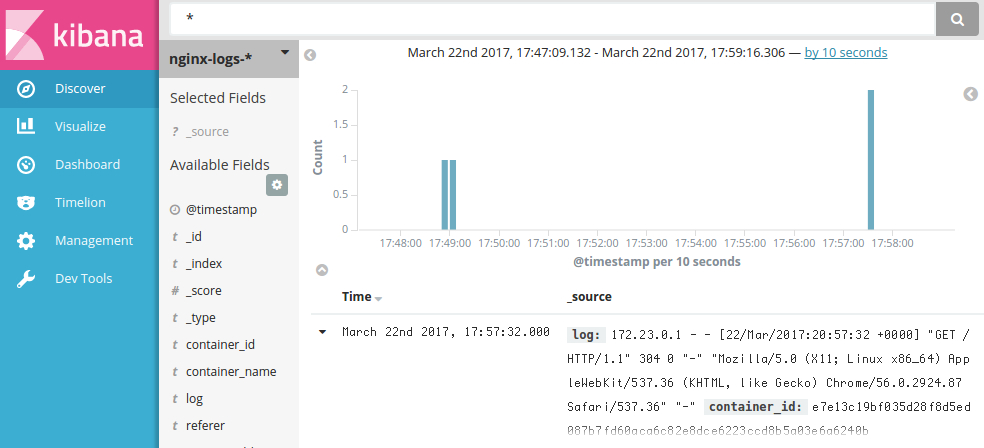
\includegraphics[width=\linewidth]{src/images/05-capitulo-5/kibanadefault.jpg}
  \caption{Cliente de \gls{term:kibana} al acceder al puerto 5601}
  \label{fig:kibana-default}
\end{figure}

Cuando se accede a \gls{term:kibana}, la página de descubrimiento se carga de
forma automática con el patrón del índice por defecto seleccionado. El filtro
de tiempo es fijado a los últimos 15 minutos y la consulta de búsqueda es
configurada para traer todos los resultados.

Es posible ver el estado de página del servidor de \gls{term:kibana}
navegando a la dirección \lstinline{localhost:5601/status}. La página de estado
(\autoref{fig:kibana-status}) muestra información acerca del uso de recursos
del servidor y lista los \eng{plugins} instalados.

\begin{figure}
  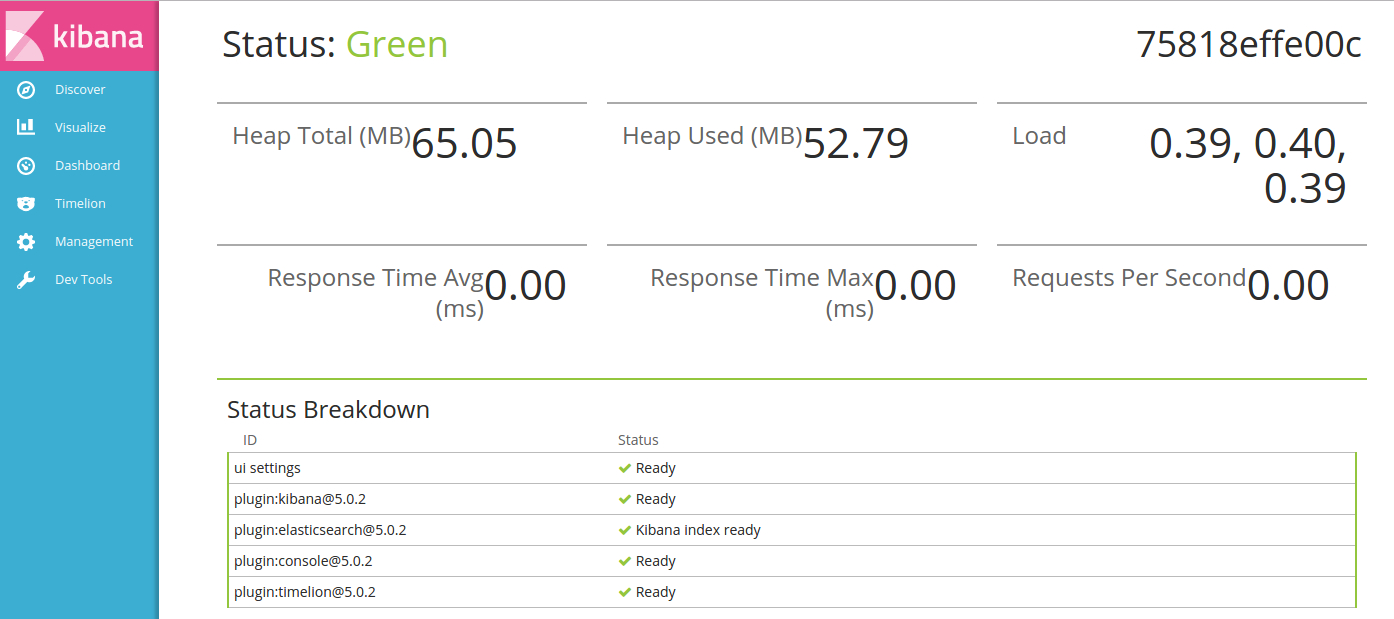
\includegraphics[width=\linewidth]{src/images/05-capitulo-5/kibanastatus.jpg}
  \caption{Vista del estado del servidor desde \gls{term:kibana}}
  \label{fig:kibana-status}
\end{figure}

Para poder comenzar a usar \gls{term:kibana}, es necesario indicar los índices
de \gls{term:elasticsearch} que se desean explorar. La primera vez que se accede
a \gls{term:kibana}, le es solicitado al usuario definir un patrón que coincida
con los nombres de uno o más índices. Una vez hecho esto ya es posible empezar a
explorar datos. En la \autoref{fig:kibana-ux} detallamos las partes de la
interfaz de \gls{term:kibana}.

Usando \gls{term:kibana} se puede realizar la exploración de datos de forma
interactiva a través de la página de descubrimiento. Desde esta página se tiene
acceso a cada documento en cada índice que coincida con un patrón de nombres de
índices seleccionado.

De esta forma, es posible enviar consultas, filtrar los resultados
de las búsquedas y visualizar datos de los documentos. Además se pueden ver los
números de documentos que coinciden con la consulta de búsqueda y obtener
estadísticas de valores de los campos.

\begin{figure}
  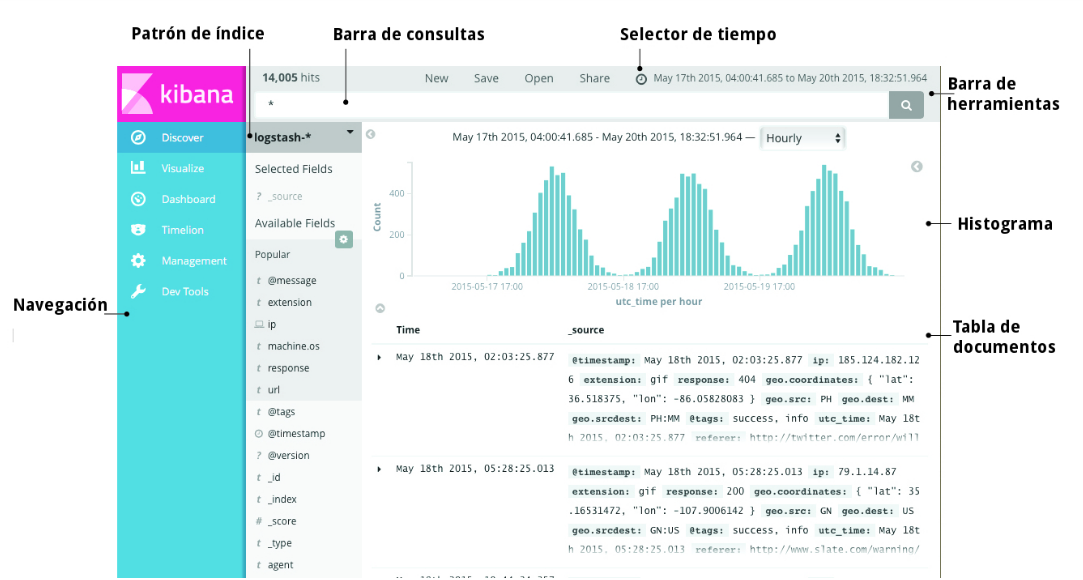
\includegraphics[width=\linewidth]{src/images/05-capitulo-5/kibana-ux.png}
  \caption{Explicación de las partes de la interfaz de \gls{term:kibana}}
  \label{fig:kibana-ux}
\end{figure}


Si un campo de tiempo es configurado para el patrón de índice seleccionado, la
distribución de documentos en el tiempo es mostrada en un \gls{term:histograma}
en la parte de arriba de la página.

\gls{term:kibana} permite crear visualizaciones de datos en los índices de
\gls{term:elasticsearch}, y con ellas construir tableros que muestren
gráficos relacionados entre sí.

Las visualizaciones de \gls{term:kibana} están basadas en consultas de
\gls{term:elasticsearch}. Al usar una serie de agregaciones de
\gls{term:elasticsearch} para extraer y procesar datos, se pueden crear
gráficos que muestren tendencias, picos y caídas, cuyo conocimiento puede ser
importante.

Es posible crear visualizaciones de distintos tipos. Algunos de estos tipos son:

\begin{itemize}

  \item \textbf{Gráficos de área:}
  Para visualizar la contribución total de varias series distintas.

  \item \textbf{Tabla de datos:}
  Para mostrar datos crudos de una agregación compuesta.

  \item \textbf{Gráfico de líneas:}
  Para comparar diferentes series.

  \item \textbf{Métrica:}
  Para mostrar un único número.

  \item \textbf{Gráfico de torta:}
  Para comparar la contribución de cada fuente.

  \item \textbf{Nube de etiquetas:}
  Para mostrar palabras de forma que el tamaño de la palabra corresponda con su importancia.

  \item \textbf{Serie de tiempo:}
  Para computar y combinar datos de múltiples conjuntos de datos de tipo serie de tiempo.

  \item \textbf{Gráfico de barras vertical:}
  Para graficar valores y comparar varias dimensiones al mismo tiempo.

\end{itemize}

El primer paso para crear una visualización es elegir el tipo de gráfico que se
quiere mostrar. Luego se debe especificar una consulta de búsqueda. Se puede
escribir una consulta nueva o tomar una búsqueda guardada anteriormente. El
siguiente paso es elegir la métrica de agregación para la visualización. Ésta
puede ser:

\begin{itemize}
  \item \textbf{count} (cantidad)
  \item \textbf{average} (promedio)
  \item \textbf{sum} (suma)
  \item \textbf{min} (mínimo)
  \item \textbf{max} (máximo)
  \item \textbf{unique count} (cantidad de elementos únicos)
  \item \textbf{median} (mediana o \gls{term:percentil} 50)
  \item \textbf{percentiles} (percentiles)
  \item \textbf{percentile ranks} (rangos de percentiles)
\end{itemize}

Además es posible agrupar los datos por fechas, rangos, términos o filtros. Por
ejemplo, si se están indexando \eng{logs} del servidor se puede construir un
gráfico de barras que muestre la distribución de solicitudes \eng{web}
entrantes por locación geográfica.

\begin{figure}
  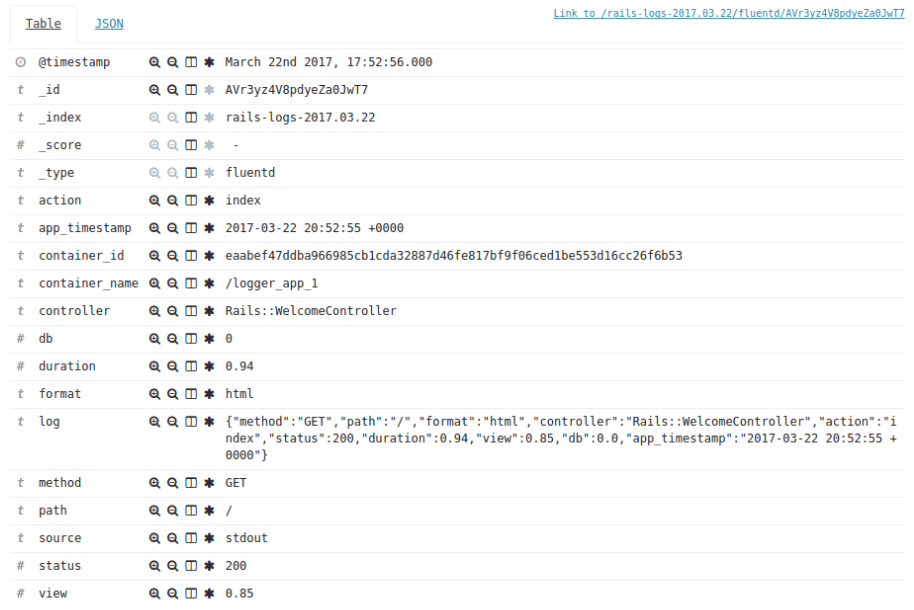
\includegraphics[width=\linewidth]{src/images/05-capitulo-5/kibana-logs.png}
  \caption{Vista de \eng{logs} de \gls{term:ror} en \gls{term:kibana}}
  \label{fig:kibana-logs}
\end{figure}

En el caso de la infraestructura \eng{web} estudiada, \gls{term:kibana} podría ser
extremadamente útil para detectar errores de forma rápida. Ante un error de una
aplicación \gls{term:ror}, se generaría un \eng{log} que sería indexado de forma
inmediata por la instancia de \gls{term:elasticsearch}.

Si realizamos una búsqueda en \gls{term:kibana} filtrando por tipo de error o
por fecha y hora, se encontraría el error en la aplicación de forma rápida
y se contaría con toda la información necesaria para reparar el error lo más
pronto posible.

En la \autoref{fig:kibana-logs} se puede ver la forma en que se visualiza en
\gls{term:kibana} una línea de \eng{logs} tomada de las aplicaciones
\gls{term:ror}. En la misma es posible apreciar cómo se ha logrado separar la
información contenida en una única línea de \eng{log} en varios atributos para
poder realizar consultas.

En este capítulo se ha mostrado cómo configurar \gls{term:kibana} para generar
tableros de control y cómo usarlo para explorar la información de \eng{logs}
almacenados en \gls{term:elasticsearch} para detectar errores de forma sencilla.

En la próxima sección se detallará cómo configurar \gls{term:grafana} para
visualizar información de la base de datos \gls{term:influx}.
